\myheading{Galois Fields, GF(2) and yet another explanation of \ac{CRC}}

\renewcommand{\CURPATH}{GF2}

\leveldown{}

\myheading{What is wrong with checksum?}

If you just sum up values of several bytes, two bit flips (increment one bit and decrement another bit) can
give the same checksum.
No good.

\myheading{Division by prime}

You can represent a file of buffer as a (big) number, then to divide it by prime.
The remainder is then very sensitive to bit flips.
For example, a prime 0x10015 (65557).

Wolfram Mathematica:

\begin{lstlisting}
In[]:= divisor=16^^10015
Out[]= 65557

In[]:= BaseForm[Mod[16^^abcdef1234567890, divisor],16]
Out[]= d8c1

In[]:= BaseForm[Mod[16^^abcdef0234567890, divisor],16]
Out[]= bd31

In[]:= BaseForm[Mod[16^^bbcdef1234567890, divisor],16]
Out[]= 382b

In[]:= BaseForm[Mod[16^^abcdee1234567890, divisor],16]
Out[]= 1fd6

In[]:= BaseForm[Mod[16^^abcdef0234567891, divisor],16]
Out[]= bd32
\end{lstlisting}

This is what is called ``avalanche effect'' in cryptography: one bit flip of input can affect many bits of output.
Go figure out which bits must be also flipped to preserve specific remainder.

You can build such a divisor in hardware, but it would require at least one adder or subtractor, you will have
a carry-ripple problem in simple case, or you would have to create more complicated circuit.

\myheading{(Binary) long divison}

Binary long division is in fact simpler then the paper-n-pencil algorithm taught in schools.

The algorithm is:

\begin{itemize}

\item 1) Allocate some ``tmp'' variable and copy dividend to it.

\item 2) Pad divisor by zero bits at left so that \ac{MSB} of divisor is at the place of \ac{MSB} of the value in tmp.

\item 3) If the divisor is larger than tmp or equal, subtract divider from tmp and add 1 bit to the quotient.
If the divisor is smaller than tmp, add 0 bit to the quotient.

\item 4) Shift divisor right.
If the divisor is 0, stop. Remainder is in tmp.

\item 5) Goto 3

\end{itemize}

The following piece of code I've copypasted from somewhere:

\begin{lstlisting}[style=customc]
unsigned int divide(unsigned int dividend, unsigned int divisor)
{
        unsigned int tmp = dividend;
        unsigned int denom = divisor;
        unsigned int current = 1;
        unsigned int answer = 0;

        if (denom > tmp)
                return 0;

        if (denom == tmp)
                return 1;

        // align divisor:
        while (denom <= tmp)
        {
                denom = denom << 1;
                current = current << 1;
        }

        denom = denom >> 1;
        current = current >> 1;

        while (current!=0)
        {
                printf ("current=%d, denom=%d\n", current, denom);
                if (tmp >= denom)
                {
                        tmp -= denom;
                        answer |= current;
                }
                current = current >> 1;
                denom = denom >> 1;
        }
        printf ("tmp/remainder=%d\n", tmp); // remainder!
        return answer;
}
\end{lstlisting}

( \url{FIXME/div.c} )

Let's divide 1234567 by 813 and find remainder:

\begin{lstlisting}
current=1024, denom=832512
current=512, denom=416256
current=256, denom=208128
current=128, denom=104064
current=64, denom=52032
current=32, denom=26016
current=16, denom=13008
current=8, denom=6504
current=4, denom=3252
current=2, denom=1626
current=1, denom=813
tmp/remainder=433
1518
\end{lstlisting}

\myheading{(Binary) long division, version 2}

Now let's say, you only need to compute a remainder, and throw away a quotient.
Also, maybe you work on some kind BigInt values and you've got a function like \TT{get\_next\_bit()} and that's it.

What we can do: tmp value will be shifted at each iteration, while divisor is not:

\begin{lstlisting}[style=customc]
uint8_t *buf;
int buf_pos;
int buf_bit_pos;

int get_bit()
{
	if (buf_pos==-1)
		return -1; // end

	int rt=(buf[buf_pos] >> buf_bit_pos) & 1;
	if (buf_bit_pos==0)
	{
		buf_pos--;
		buf_bit_pos=7;
	}
	else
		buf_bit_pos--;
	return rt;
};

uint32_t remainder_arith(uint32_t dividend, uint32_t divisor)
{
	buf=(uint8_t*)&dividend;
	buf_pos=3;
	buf_bit_pos=7;

	uint32_t tmp=0;

	for(;;)
	{
		int bit=get_bit();
		if (bit==-1)
		{
			printf ("exit. remainder=%d\n", tmp);
			return tmp;
		};

		tmp=tmp<<1;
		tmp=tmp|bit;

		if (tmp>=divisor)
		{
			printf ("%d greater or equal to %d\n", tmp, divisor);
			tmp=tmp-divisor;
			printf ("new tmp=%d\n", tmp);
		}
		else
			printf ("tmp=%d, can't subtract\n", tmp);
	};
}
\end{lstlisting}

( \url{FIXME/div_both.c} )
	
Let's divide 1234567 by 813 and find remainder:

\lstinputlisting{\CURPATH/log.txt}

\myheading{Shortest possible introduction into GF(2)}

There is a difference between digit and number.
Digit is a symbol, number is a group of digits.
0 can be both digit and number.

Binary digits are 0 and 1, but a binary number can be any.

There are just two numbers in Galois Field (2): 0 and 1.
No other numbers.

What practical would you do with just two numbers?
Not much, but you can pack GF(2) numbers into some kind of structure or tuple or even array.
Such structures are represented using polynomials.
For example, CRC32 polynomial you can find in source code is 0x04C11DB7.
Each bit represent a number in GF(2), not a digit.
The 0x04C11DB7 polynomial is written as: 

$x^{32} + x^{26} + x^{23} + x^{22} + x^{16} + x^{12} + x^{11} + x^{10} + x^8 + x^7 + x^5 + x^4 + x^2 + x + 1$

Wherever $x^n$ is present, that means, you have a bit at position $n$.
Just $x$ means, bit present at LSB.
There is, however, bit at $x^{32}$, so the CRC32 polynomial has the size of 33 bits, bit the \ac{MSB} is always 1 and is
omitted in all algorithms.

It's important to say that unlike in algebra, GF(2) polynomials are never evaluated here.
$x$ is symbol is present mereley as a convention.
People represent GF(2) "structures" as polynomials to emphasize the fact that "numbers" are isolated from each other.

Now, subtraction and addition are the same operations in GF(2) and actually works as XOR.
This is present in many tutorials, so I'll omit this here.

Also, by convention, whenever you compare two numbers in GF(2), you only compare two most significant bits,
and ignore the rest.

\myheading{CRC32}

Now we can take the binary division algorithm and change it a little:

\begin{lstlisting}[style=customc]
uint32_t remainder_GF2(uint32_t dividend, uint32_t divisor)
{
	// necessary bit shuffling/negation to make it compatible with other CRC32 implementations.
	// N.B.: input data is not an array, but a 32-bit integer, hence we need to swap endiannes.
	uint32_t dividend_negated_swapped = ~swap_endianness32(bitrev32(dividend));
	buf=(uint8_t*)&dividend_negated_swapped;
	buf_pos=3;
	buf_bit_pos=7;

	uint32_t tmp=0;

	// process 32 bits from the input + 32 zero bits:
	for(int i=0; i<32+32; i++)
	{
		int bit=get_bit();
		int shifted_bit=tmp>>31;

		// fetch next bit:
		tmp=tmp<<1;
		if (bit==-1)
		{
			// no more bits, but continue, we fetch 32 more zero bits.
			// shift left operation set leftmost bit to zero.
		}
		else
		{
			// append next bit at right:
			tmp=tmp|bit;
		};

		// at this point, tmp variable/value has 33 bits: shifted_bit + tmp
		// now take the most significant bit (33th) and test it:
		// 33th bit of polynomial (not present in "divisor" variable is always 1
		// so we have to only check shifted_bit value
		if (shifted_bit)
		{
			// use only 32 bits of polynomial, ingore 33th bit, which is always 1:
			tmp=tmp^divisor;
		};
	};
	// bit shuffling/negation for compatibility once again:
	return ~bitrev32(tmp);
}
\end{lstlisting}

( \url{FIXME/div_both.c} )

And voila, this is the function which computes CRC32 for the input 32-bit value.

There are only 3 significant changes:

\begin{itemize}
\item XOR instead of minus.

\item Only \ac{MSB} is checked during comparison. But the \ac{MSB} of all CRC polynomials is always 1,
so we only need to check \ac{MSB} (33th bit) of the tmp variable.

\item There are 32+32=64 iterations instead of 32.
As you can see, only \ac{MSB} of tmp affects the whole behaviour of the algorithm.
So when tmp variable is filled by 32 bits which never affected anything so far,
we need to "blow out" all these bits through 33th bit of tmp variable to get correct remainder (or CRC32 sum).
\end{itemize}

All the rest algorithms you can find on the Internet are optimized version, which may be harder to understand.
No algorithms used in practice ``blows'' anything ``out'' due to optimization.
Many practical algorithms are either bytewise (process input stream by bytes, not by bits) or table-based.

My goal was to write two functions, as similar to each other as possible, to demonstrate the difference.

So the CRC value is in fact remainder of division of input date by CRC polynomial in GF(2) environment.
As simple as that.

\myheading{Rationale}

Why would anyone use such an unusual mathematics?
The answer is: many GF(2) operations can be done using bit shifts and XOR, which are very cheap operations.

Electronic circuit for CRC generator is extremely simple, it consists of only shift register and XOR gates.
This one is for CRC16:

% TODO: TikZ?
\begin{figure}[H]
\centering
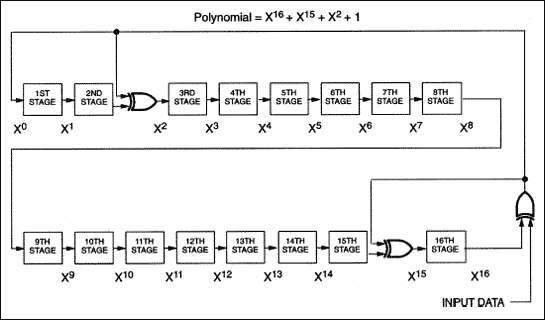
\includegraphics[scale=1]{\CURPATH/CRC16.png}
\caption{}
\end{figure}

( The source of image: \url{https://olimex.wordpress.com/2014/01/10/weekend-programming-challenge-week-39-crc-16/} )

Only 3 XOR gates are present aside of shift register.

The following page has animation: \url{https://en.wikipedia.org/wiki/Computation_of_cyclic_redundancy_checks}.

It can be implemented maybe even using vacuum tubes.

And the task is not to compute remainder according to rules of arithmetics, but rather to detect errors.

Compare this to a division circuit with at least one binary adder/subtractor, which will have carry-ripple problem.
On the other hand, addition over GF(2) has no carries, hence, this problem absent.

\myheading{Further reading}

These documents I've found interesting/helpful:

\begin{itemize}

\item \url{http://www.ross.net/crc/download/crc_v3.txt}
\item \url{https://www.kernel.org/doc/Documentation/crc32.txt}
\item \url{http://web.archive.org/web/20161220015646/http://www.hackersdelight.org/crc.pdf}

\end{itemize}

\levelup{}

